\section{Potenzfunktionen}\index{Funktion!Potenzfunktionen}\index{Potenzfunktionen}
\sectuntertitel{Funktionen hoch drei!}

\subsection*{Lernziele}

\begin{itemize}
\item Definition Ganzzahlige Potenzfunktion
\item Graphische Darstellung
\end{itemize}
\newpage


\subsection{Einstieg}
\subsubsection{Beispiel: Reinquadratische Funktion}\index{quadratische Funktion}\index{Funktion!quadratische}

Zeichnen Sie den Graphen der Funktion $f: y= \frac16 x^2$:

\bbwGraph{-7}{7}{-1}{6.5}{%%
  \TRAINER{
    \bbwFunc{\x*\x/6}{-6:6}
  }
}%%

\begin{definition}{Reinquadratische Funktion}{}
Die Funktion

$f: y = a\cdot{}x^2$

heißt rein-quadratische Funktion.
\end{definition}


\begin{bemerkung}{}{}
Eine allgemeine quadratische Funktion besitzt auch noch einen linearen ($bx$) und einen konstanten ($c$) Anteil. Die allgemeine quadratische Funktion hat die Form

$$f: y= ax^2 + bx + c$$
\end{bemerkung}


\GESO{Beispiele zu allgemeinen quadratischen Funktionen finden sie im Buch \cite{marthaler21} ab Seite 260 insb. im Bild zu Aufg. 4 auf Seite 273.}

\GESO{\subsection*{Aufgaben}}
\GESOAadB{303ff}{1. (nur $n=3$ und $n=5$), 2. (nur $n=4$ und $n=6$)}

\newpage
%%%%%%%%%%%%%%%%%%%%%%%%%%%%%%%%%%%%%%%%%%%%%%%%%%%%%%%%%%%%%%%%%
\subsubsection{Beispiel: Polynomfunktionen\GESO{ (optional)}}

Betrachten wir einmal die (Polynom-)Funktion $f: y = 0.1x^3 + x^2 + 2x + 3 - x^{-1}$ \zB mit Geogebra (\texttt{www.geogebra.org}).

\bbwGraph{-10}{4}{-7}{8}{%
  \bbwFunc{0.1*\x*\x*\x + \x*\x + 2*\x + 3 -1/\x}{-8.5:-0.2}
  \bbwFunc{0.1*\x*\x*\x + \x*\x + 2*\x + 3 -1/\x}{0.1:1.5}
}%%


Polynomfunktionen sind «\textit{weiche}» Funktionen, die jedoch \textbf{Asymptoten}\index{Asymptote} (hier bei $x=0$) aufweisen können.
Ebenso sind die Extremwerte (lokale Maxima und Minima) wie auch die Wendepunkte charakteristische Stellen und oft Gegenstand der Untersuchung.
Wir beschränken und auf Potenzfunktionen der Art $f: y=a\cdot{}x^z$
mit $z \in \mathbb{Z}\backslash\{0\}$. \textbf{Potenzfunktionen} sind
Polynomfunktionen, bei denen nur ein Summand vorkommt.
\newpage


\subsection{Parabel}\index{Parabel}

\begin{definition}{Parabel}{definition_parabel}
  Eine Funktion der Art
$$f: y=a\cdot{}x^n$$
mit $n \in \mathbb{N}$ heißt \textbf{Parabel} $n$-ter Ordnung.\index{Parabel}
\end{definition}

Zeichnen Sie $y = \frac{1}{16}x^4$ im Bereich $[-3; 3]$ indem Sie für jeden 0.5-er $x$-Wert das zugehörige $y$ berechnen:

\bbwGraph{-4}{4}{-1}{6.5}{%%
  \TRAINER{\bbwFunc{\x*\x*\x*\x/16}{-3:3}}
}%%
\newpage

Zeichnen Sie des weiteren die Funktion $y = \frac{1}{9}x^3$:

\bbwGraph{-4}{4}{-6}{6}{%%
  \TRAINER{\bbwFunc{\x*\x*\x/9}{-3.5:3.5}}
}%%

Was fällt für gerade und ungerade Exponenten auf? Gibt es Spiegelachsen
oder Spiegelpunkte?

\renewcommand{\mmPapier}[1]{\mmPapierZwei{#1}{16.4}}
\begin{tabular}{c|p{8cm}}
  $x$ &  \TNT{0.8}{Am Ursprung $O(0|0)$}\\
  \hline
  $x^2$ &  \TNT{0.8}{An der $y$-Achse}\\
  \hline
  $x^3$ &  \TNT{0.8}{Am Ursprung $O(0|0)$}\\
  \hline
  $x^4$ &  \TNT{0.8}{An der $y$-Achse}\\
  \hline
  
\end{tabular}
\renewcommand{\mmPapier}[1]{\mmPapierZwei{#1}{17.6}}


\GESO{Eine Zusammenfassung der wichtigsten Eigenschaften von
  Potenzfunktionen finden Sie im Buch \cite{marthaler21} Seite 296 oben.}
\newpage

\subsubsection{Referenzaufgabe}

Bestimmen Sie $a$ und $k$ so, dass der Graph von $y = a \cdot{} x^k$
durch die Punkte $P=\left(3 \middle| 1458\right)$ und
$Q=\left(-4\middle|8192\right)$ verläuft.

\TNT{13.2}{  Punkte einsetzen in die Funktionsgleichung:
  \gleichungZZ{1458}{a\cdot{}3^k}{8192}{a\cdot{}(-4)^k}
  Aus der oberen Gleichung das $a$ ermitteln ($a=\frac{1485}{3^k}$)
  (I) und in die zweite
  Gleichung einsetzen: $$8192 = \frac{1458}{3^k} \cdot{} (-4) ^k$$
  Exponent $k$ separieren:
  $$\frac{8192}{1458} = \left(\frac{-4}3\right)^k$$
  Problem: Logarithmen mit negativen Basen (hier $\frac{-4}3$)
  funktionieren nicht!
  
  Weil nun $k$ gerade sein muss folgt, dass $\left(\frac{-4}3\right)^k
  = \left(\frac43\right)^k$. Daraus ergibt sich
  $$\frac{8192}{1458} = \left(\frac{4}3\right)^k \Longrightarrow k =
  \log_{\frac43}\left(\frac{8192}{1485}\right) = 6$$
  Dieses $k$ nun in die Gleichung (I) einsetzen; dies
  liefert
  $$a=\frac{1458}{3^k} = 2.$$
}%% end TRAINER


\subsection*{Aufgaben}
\GESOAadB{305ff}{11. a) b) c), 13. a) c), (optional 17.,)  18.}
\TALSAadB{197}{736. b), 737. a) c)}
\newpage


\subsection{Translationen}\index{Manipulation!Funktionen}\index{Funktions-Manipulation}\index{Translation!Funktion}
\sectuntertitel{Manipulation an Funktionsgraphen}
(Verschiebung\index{Verschiebung}, Spiegelung\index{Spiegelung},
Streckung\index{Streckung})

\theorieGESO{227}{13.3}
\theorieTALS{163}{3}

Wir betrachten die verschiedenen geometrischen
Funktions-«Manipulationen» (Abbildungen) am Beispiel {\color{red}$y =f(x) = \frac18 x^3$}.

\leserluft{}

\newcommand{\graphTranslationMultiColumn}[5]{%
  \multicolumn{3}{|l|}{#1}\\%%
\hline%%
\graphTranslationMultiColumnZ{#2}{#3}{#4}{#5}
}%% end new command \graphTranslationMultiColumn

\newcommand{\graphTranslationMultiColumnZ}[4]{%
\multirow{5}{6cm}{#1} &  & \multirow{2}{*}{\begin{minipage}{.3\textwidth}\raisebox{-8cm}{\includegraphics[width=\linewidth,height=60mm]{allg/funktionen/img/translation/#4}}\end{minipage}}\\[55mm]%%
&\fbox{#2}&\\%%
&&\\%%
&{\color{red}\fbox{#3}}&\\%%
&&\\%%
\hline%%
}%% end new command \graphTranslationMultiColumnZ


\begin{tabular}{|p{7cm}|c|c|}%%
\hline%%
\graphTranslationMultiColumn{Verschiebung in $y$-Richtung...}{... um \textbf{zwei} Einheiten nach \textbf{oben}:}{$g(x)=f(x)\textbf{+2}$}{$g(x)=\frac18x^3\textbf{+2}$}{typ1.png}
\graphTranslationMultiColumnZ{... um \textbf{eine} Einheiten nach \textbf{unten}:}{$g(x)=f(x)\textbf{-1}$}{$g(x)=\frac18x^3\textbf{-1}$}{typ2.png}
\end{tabular}%%

\begin{tabular}{|p{7cm}|c|c|}%%
\hline%%
\graphTranslationMultiColumn{Spiegelung...}{... an der $x$-Achse:}{$g(x)=-f(x)$}{$g(x)=-\frac18x^3$}{typ3.png}
\graphTranslationMultiColumnZ{... an der $y$-Achse:}{$g(x)=f(-x)$}{$g(x)=\frac18(-x)^3$}{typ4.png}
\end{tabular}%%

\begin{tabular}{|p{7cm}|c|c|}%%
\hline%%
\graphTranslationMultiColumn{Streckung...}{... in $y$-Richtung (von der $x$-Achse aus) um Faktor \textbf{zwei}:}{$g(x)=\textbf{2}\cdot{}f(x)$}{$g(x)=\textbf{2}\cdot{}\frac18x^3$}{typ5.png}
\graphTranslationMultiColumnZ{... in $x$-Richtung (von der $y$-Achse aus) um Faktor \textbf{zwei}:}{$g(x)=f(\frac{1}{\textbf{2}}\cdot{}x)$}{$g(x)=\frac18(\frac{1}{\textbf{2}}\cdot{}x)^3$}{typ6.png}
\end{tabular}%%

\TALS{%% Nur TALS verschieben in x-Richtung
\begin{tabular}{|p{7cm}|c|c|}%%
\hline%%
\graphTranslationMultiColumn{Verschiebung in $x$-Richtung\footnote{Kein prüfungsrelevantes Thema.}...}{... um \textbf{zwei} Einheiten nach \textbf{links}:}{$g(x)=f(x\textbf{+2})$}{$g(x)=\frac18(x\textbf{+2})^3$}{typ7.png}
\graphTranslationMultiColumnZ{... um \textbf{zwei} Einheiten nach \textbf{rechts}:}{$g(x)=f(x\textbf{-2})$}{$g(x)=\frac18(x\textbf{-2})^3$}{typ8.png}
\end{tabular}%%
}%% END TALS
\newpage

Skizzieren Sie $-\frac{1}{2}x^3 - 1$ im Bereich $x$ = -2 bis $x$ = +2.

\bbwGraph{-4}{4}{-5}{3}{%%
  \TRAINER{%
    \bbwFunc{-0.5*\x*\x*\x-1}{-2:2}%
  }%%
}%



\subsection*{Aufgaben}
\GESOAadB{304ff}{5. a) c) d) e), 9. a) d) e)}

\aufgabenfarbe{Arbeitsblatt im OLAT «Positive Potenzfunktionen
  zuordnen»}
\TALSAadB{197}{738., 739.}
\newpage

%%%%%%%%%%%%%%%%%%%%%%%%%%%%%%%%%%%%%%%%%%%%%%%%%%%%%%%%%%%%%%%%%%%%%%%%%%%%%%%%%%%
\subsection{Hyperbel}\index{Hyperbel (negative Exponenten)}
(«Hyperbel» Griechisch = «über das Ziel hinaus werfen»)


Zur Erinnerung:
\begin{multicols}{2}
\begin{itemize}
	\item $x^{-1} = \frac{1}{x}$
	\item $x^{-2} = \frac{1}{x^2}$
	\item $x^{-3} = \frac{1}{x^3}$
	\item $x^{-4} = \frac{1}{x^4}$
	\item $x^{-5} = \frac{1}{x^5}$
  \item ...
\end{itemize}
\end{multicols}

Zeichnen Sie die Funktion $f: y = x^{-1}$ im Bereich $[-5;5]$:

\bbwGraph{-6}{6}{-3}{3}{%%
  \TRAINER{\bbwFunc{1/\x}{-5:-0.3}}
  \TRAINER{\bbwFunc{1/\x}{0.3:5}}

}%%

\newpage


Zeichnen Sie zusätzlich Funktion $f: y = x^{-2}$  und $x^{-3}$im Bereich $[-5;5]$:

\bbwGraph{-6}{6}{-5}{5}{%%
  % x^-2
  \TRAINER{\bbwFuncC{1/(\x * \x)}{-5:-0.447}{green}}%% 0.447 = 1/sqrt (5)
  \TRAINER{\bbwFuncC{1/(\x * \x)}{0.447:5}{green}}
  \TRAINER{\bbwLetter{2.5,0.5}{x^{-2}}{green}}
  \TRAINER{\bbwLetter{-1.5,1}{x^{-2}}{green}}

  %x^-3
  \TRAINER{\bbwFuncC{1/(\x * \x * \x)}{-5:-0.584}{blue}}
  \TRAINER{\bbwFuncC{1/(\x * \x * \x)}{0.584:5}{blue}}
  \TRAINER{\bbwLetter{0.8,0.3}{x^{-3}}{blue}}
  \TRAINER{\bbwLetter{-1.2,-3.8}{x^{-3}}{blue}}
  \TRAINER{\bbwLetter{1.2,4.5}{x^{-3}}{blue}}

}%%

\begin{definition}{Hyperbel}{definition_hyperbel}
  Eine Funktion $$f: y=ax^z$$
  mit $z \in \{-1, -2, -3, -4, ...\}$ heißt
\textbf{Hyperbel}\index{Hyperbel} der Ordnung $z$.
\end{definition}

Der Definitionsbereich von Hyperbeln entspricht dem Definitionsbereich
des Funktionsterms. Merke: Es darf nicht durch Null geteilt werden:

$$x^{-5} = \frac{1}{x^5} \Longrightarrow \mathbb{D} = \mathbb{R} \backslash \{0\}$$


\subsection*{Aufgaben}
\GESOAadB{306ff}{19. Zeichnung mit geogebra.org, 20.
  Zeichnung mit geogebra.org, 25. b) c), 26. a) b), 27. b) c), 33*}
\TALSAadB{205}{771. a) c) d) e) g) h) j)}


\newpage

\subsubsection{Charakteristiken}
\textbf{Spiegelungen:}\\

Welche Funktionen $x$, $x^{-1}$, $x^{-2}$, $x^{-3}$ sind an welchen Achsen bzw. Punkten gespiegelt?

\renewcommand{\mmPapier}[1]{\mmPapierZwei{#1}{16.0}}
\begin{tabular}{c|p{10cm}}
  $x$     &  \TNT{0.8}{Am Ursprung $O(0|0)$ : Punktspiegelung}\\
  \hline
  $x^{-1}$ &  \TNT{0.8}{Am Ursprung $O(0|0)$ : Punktspiegelung}\\
  \hline
  $x^{-2}$ &  \TNT{0.8}{An der $y$-Achse: Achsensymmetrie}\\
  \hline
  $x^{-3}$ &  \TNT{0.8}{Am Ursprung $O(0|0)$: Punktspiegelung}\\
  \hline
  $x^{-4}$ &  \TNT{0.8}{An der $y$-Achse: Achsensymmetrie}\\
  \hline  
\end{tabular}
\renewcommand{\mmPapier}[1]{\mmPapierZwei{#1}{17.6}}


\paragraph{Definitions- und Wertebereiche:}

Geben Sie für die obigen Funktionen an, was ihr Definitions- bzw. Wertebereich ist\footnote{Grundmenge ist $\mathbb{R}$.}:

\begin{tabular}{c|c|c}
Funktionsterm & Definitionsbereich $\mathbb{D}$& Wertebereich $\mathbb{W}$\\ \hline
  $x$     & \TRAINER{$\mathbb{R}$} &  \TRAINER{$\mathbb{R}$}\\ \hline
  $x^{-1}$ & \TRAINER{$\mathbb{R}\backslash\{0\}$} &  \TRAINER{$\mathbb{R}\backslash\{0\}$}\\ \hline
  $x^{-2}$ & \TRAINER{$\mathbb{R}\backslash\{0\}$} &  \TRAINER{$\mathbb{R}^{+}\backslash\{0\}$}\\ \hline
  $x^{-3}$ & \TRAINER{$\mathbb{R}\backslash\{0\}$} &  \TRAINER{$\mathbb{R}\backslash\{0\}$}\\ \hline
  $x^{-4}$ & \TRAINER{$\mathbb{R}\backslash\{0\}$} &  \TRAINER{$\mathbb{R}^{+}\backslash\{0\}$}\\ \hline
\end{tabular}


\subsection*{Aufgaben}
\GESO{\aufgabenfarbe{Weitere Aufgaben im \textit{Kompendium} Kap. 3.3 S. 26. Aufg. 28-31}}
\GESO{\aufgabenfarbe{Aufgabe der Nullserie 2 (zweite Nullserie): Aufg. 7 auf Seite 3}}
\GESO{\aufgabenfarbe{Maturaprüfung 2016, Aufg. 8 (Graphen zuordnen)}}
\newpage

\subsection{Zusammenfassungen und
  Überblick}\index{Potenzfunktionen!Überblick}

$$y = a\cdot{}x^z$$

$z$ gerade: Gespiegelt an der $y$-Achse

$z$ ungerade: Gespiegelt am Ursprung $O=(0|0)$

Ist ${\color{green}a>0}$\TRAINER{ (grün in der Graphik)}, so sind Graphen mit
geraden Exponenten nach oben geöffnet bzw. mit ungeraden Exponenten im
Quadranten I und III.

Ist ${\color{red}a<0}$\TRAINER{ (rot/orange in der Graphik)}, so sind Graphen mit
geraden Exponenten nach unten geöffnet bzw. mit ungeraden Exponenten
im Quadranten II und IV.

\TNT{8}{
 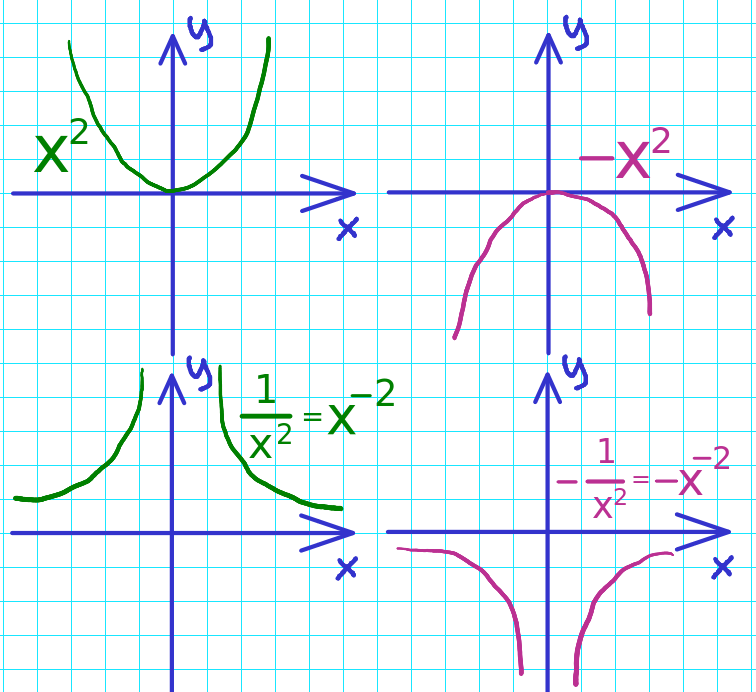
\includegraphics[width=8.5cm]{allg/funktionen/img/potenzfct/potenzFunktionenGerade.png}\hfill{}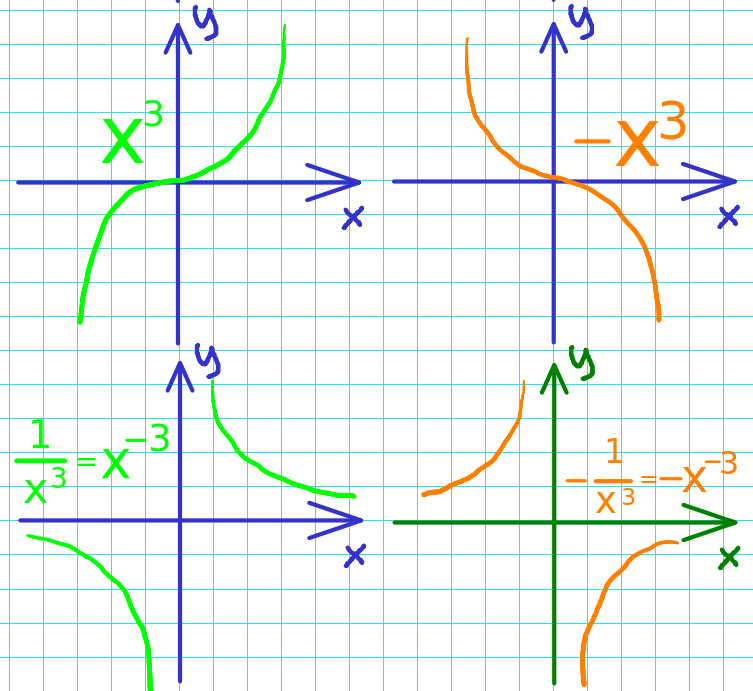
\includegraphics[width=8.5cm]{allg/funktionen/img/potenzfct/potenzFunktionenUngerade.png}
}%% END TNT
\newpage
